\documentclass[11pt,a4paper]{article}

% --- Packages ---
\usepackage[utf8]{inputenc}
\usepackage[margin=1in]{geometry}
\usepackage{helvet}
\renewcommand{\familydefault}{\sfdefault}
\usepackage{amsmath,amssymb}
\usepackage{graphicx}
\usepackage{xcolor}
\usepackage{booktabs}
\usepackage{tabularx}
\usepackage{array}
\usepackage{listings}
\usepackage{tikz}
\usetikzlibrary{shapes.geometric, arrows, positioning, shadows, calc}
\usepackage{tcolorbox}
\tcbuselibrary{skins, breakable}
\usepackage{fancyhdr}
\usepackage[hidelinks,colorlinks=true,linkcolor=blue,urlcolor=cyan,citecolor=blue]{hyperref}

% --- Color Definitions ---
\definecolor{primaryblue}{RGB}{0, 102, 204}
\definecolor{darknavy}{RGB}{13, 21, 38}
\definecolor{accentcyan}{RGB}{0, 180, 216}
\definecolor{lightgrey}{RGB}{245, 247, 250}
\definecolor{bordergrey}{RGB}{220, 224, 230}
\definecolor{codebg}{RGB}{240, 243, 246}
\definecolor{warnred}{RGB}{220, 53, 69}
\definecolor{tipgreen}{RGB}{40, 167, 69}

% --- Callout Box Styles ---
\newtcolorbox{importantbox}[1][]{
  colback=warnred!10!white,
  colframe=warnred,
  fonttitle=\bfseries,
  coltitle=white,
  title=CRITICAL SYSTEM FAILSAFE RULES,
  enhanced,
  attach boxed title to top left={xshift=10pt, yshift=-10pt},
  boxed title style={colback=warnred},
  #1
}

\newtcolorbox{tipbox}[1][]{
  colback=tipgreen!10!white,
  colframe=tipgreen,
  fonttitle=\bfseries,
  coltitle=white,
  title=ADVANCED FEATURE: Direct PC MicroSD Access,
  enhanced,
  attach boxed title to top left={xshift=10pt, yshift=-10pt},
  boxed title style={colback=tipgreen},
  #1
}

% --- Listings Configuration ---
\lstset{
  backgroundcolor=\color{codebg},
  basicstyle=\ttfamily\small,
  breaklines=true,
  captionpos=b,
  commentstyle=\color{gray},
  keywordstyle=\color{primaryblue}\bfseries,
  stringstyle=\color{accentcyan},
  frame=single,
  rulecolor=\color{bordergrey},
  showstringspaces=false
}

% --- Header and Footer ---
\pagestyle{fancy}
\fancyhf{}
\lhead{\textbf{AUV Detailed Technical Reference \& Operational Manual}}
\rhead{ESP32-S3 Suite}
\cfoot{\thepage}

\title{\textbf{\Huge Autonomous Underwater Vehicle (AUV)}\\[0.3em]
\Large Complete Embedded System Engineering Manual \& Software Architecture Guide}
\author{\textbf{Autonomous Control \& Avionics Group}}
\date{\today}

\begin{document}

\maketitle

\begin{abstract}
This engineering reference manual provides an exhaustive, highly detailed breakdown of the Autonomous Underwater Vehicle (AUV) embedded electronics hardware, software architecture, multi-core FreeRTOS task scheduling, CAN bus identifier mapping, binary ESP-NOW message schemas, fail-safe recovery logic, 3D web ground station mechanics, and operational procedures. The suite is built upon four (4) ESP32-S3 microcontrollers linked via a 500~kbps Two-Wire Automotive Interface (TWAI) CAN Bus, an ESP-NOW 2.4~GHz radio mesh, and a dual USB-Serial / Wi-Fi WebSockets ground station interface.
\end{abstract}

\tableofcontents
\newpage

% =========================================================
\section{System Engineering Overview}
% =========================================================

The AUV onboard avionics suite employs a \textbf{distributed multi-microcontroller architecture} designed for maximum reliability, high throughput, and real-time responsiveness under harsh marine environments. The system divides perception, motor actuation, central telemetry management, and wireless ground communication across four dedicated ESP32-S3 32-bit dual-core processors running FreeRTOS.

\begin{figure}[htbp]
\centering
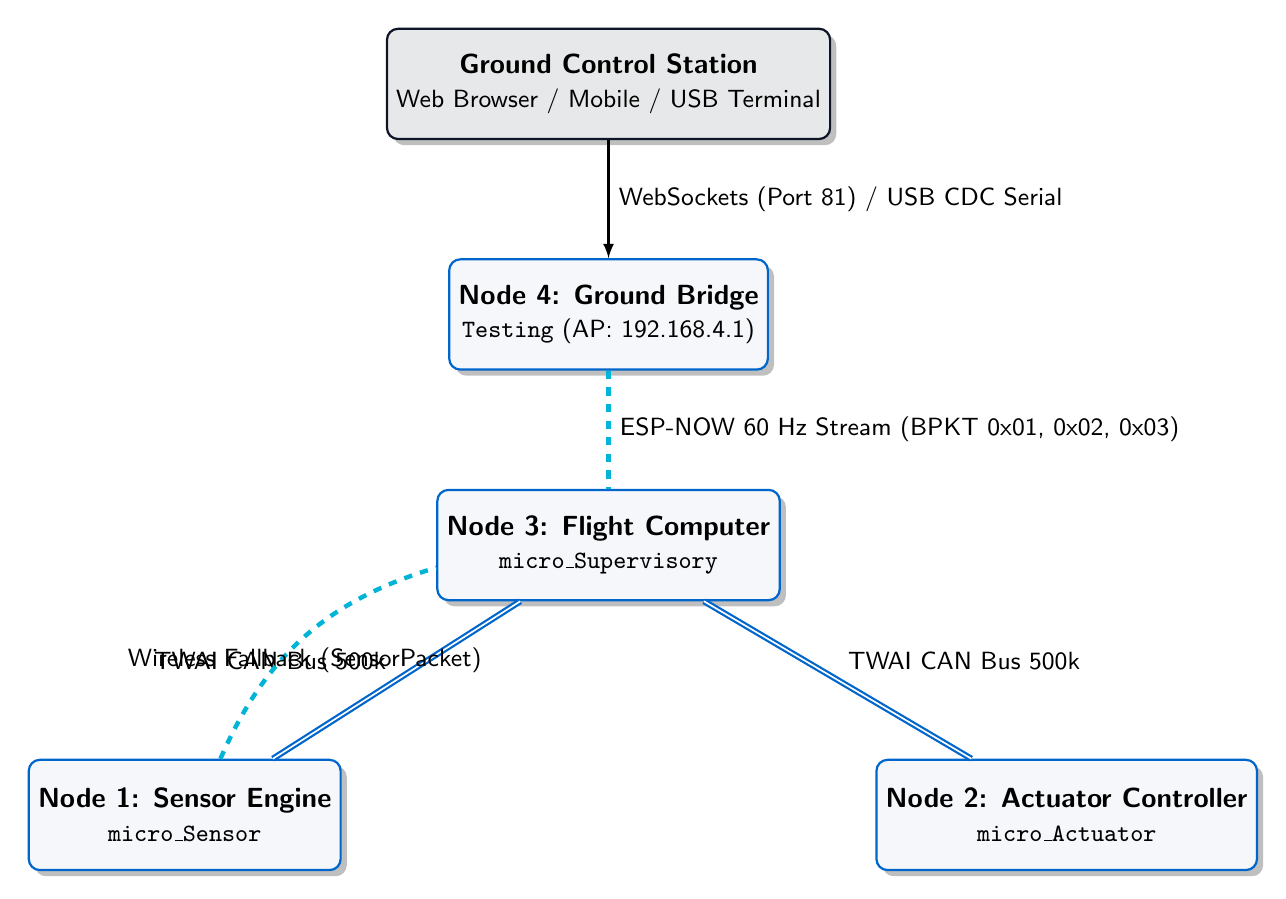
\begin{tikzpicture}[
    node distance=1.5cm and 2cm,
    block/.style={rectangle, draw=primaryblue, fill=lightgrey, thick, rounded corners, align=center, minimum width=3.4cm, minimum height=1.4cm, drop shadow},
    gsblock/.style={rectangle, draw=darknavy, fill=darknavy!10, thick, rounded corners, align=center, minimum width=3.8cm, minimum height=1.4cm, drop shadow},
    line/.style={draw, -latex, thick},
    canline/.style={draw=primaryblue, double, thick},
    espline/.style={draw=accentcyan, dashed, ultra thick}
]

% Nodes
\node [gsblock] (gs) {\textbf{Ground Control Station}\\\small Web Browser / Mobile / USB Terminal};
\node [block, below=of gs] (br) {\textbf{Node 4: Ground Bridge}\\\small\texttt{Testing} (AP: 192.168.4.1)};
\node [block, below=of br] (sup) {\textbf{Node 3: Flight Computer}\\\small\texttt{micro\_Supervisory}};
\node [block, below left=2cm and 1.2cm of sup] (sen) {\textbf{Node 1: Sensor Engine}\\\small\texttt{micro\_Sensor}};
\node [block, below right=2cm and 1.2cm of sup] (act) {\textbf{Node 2: Actuator Controller}\\\small\texttt{micro\_Actuator}};

% Connectors
\path [line] (gs) -- node[right]{\small WebSockets (Port 81) / USB CDC Serial} (br);
\path [espline] (br) -- node[right]{\small ESP-NOW 60 Hz Stream (BPKT 0x01, 0x02, 0x03)} (sup);
\path [canline] (sup) -- node[above left]{\small TWAI CAN Bus 500k} (sen);
\path [canline] (sup) -- node[above right]{\small TWAI CAN Bus 500k} (act);
\path [espline, bend left=25] (sen) to node[below]{\small Wireless Fallback (SensorPacket)} (sup);

\end{tikzpicture}
\caption{System Hardware Network Topology, Bus Architecture, and Inter-Node Interfaces.}
\label{fig:network_topology}
\end{figure}

---

% =========================================================
\section{Microcontroller Node Engineering \& Hardware Pinouts}
% =========================================================

\subsection{Node 1: \texttt{micro\_Sensor} (Navigation \& Perception Engine)}
Node 1 acts as the vehicle's primary perception unit. It acquires data from a 9-DOF IMU, a multi-GNSS receiver, an underwater ultrasonic transducer, and an analog pressure depth sensor.

\begin{itemize}
    \item \textbf{Firmware File:} \href{file:///c:/Users/MP2KC/OneDrive/Documents/PlatformIO/Projects/micro_Sensor/src/main.cpp}{\texttt{micro\_Sensor/src/main.cpp}}
    \item \textbf{PlatformIO File:} \href{file:///c:/Users/MP2KC/OneDrive/Documents/PlatformIO/Projects/micro_Sensor/platformio.ini}{\texttt{micro\_Sensor/platformio.ini}}
\end{itemize}

\subsubsection{Peripherals \& Electrical Interfacing}
\begin{enumerate}
    \item \textbf{BNO055 9-DOF IMU (I2C):} Connected to I2C bus (\texttt{SDA: GPIO 38}, \texttt{SCL: GPIO 39}) operating at 100~kHz. Measures absolute orientation (Euler angles: Pitch, Roll, Yaw) fused via internal ARM Cortex-M0 core.
    \item \textbf{ATGM336H GPS Receiver (UART1):} Connected to Hardware Serial 1 (\texttt{RX: GPIO 17}, \texttt{TX: GPIO 18}) at 9600 baud. Parsed continuously using \texttt{TinyGPS++} for Latitude, Longitude, Altitude, Speed, HDOP, Satellites, and UTC time.
    \item \textbf{Underwater Ultrasonic Sonar Transducer (UART2):} Connected to Hardware Serial 2 (\texttt{RX: GPIO 16}, \texttt{TX: GPIO 15}) at 9600 baud. Parses 4-byte binary frames \texttt{[0xFF, High, Low, Checksum]} where:
    \begin{equation}
        \text{Checksum} = (\text{0xFF} + \text{High} + \text{Low}) \pmod{256}
    \end{equation}
    Distance in millimeters is calculated as: $\text{Distance (mm)} = (\text{High} \ll 8) \mid \text{Low}$.
    \item \textbf{4--20~mA Pressure Depth Sensor (ADC1):} Submersible depth sensor connected to ADC1 pin \texttt{GPIO 13} with 11~dB attenuation (0--3.3~V input range) and 12-bit resolution (0--4095). Applies an 8-sample moving average filter:
    \begin{equation}
        V_{\text{avg}} = \frac{1}{8} \sum_{i=1}^{8} \text{ADC}_i \times \frac{3.3}{4095}, \quad \text{Depth (mm)} = V_{\text{avg}} \times \frac{5000.0}{3.3}
    \end{equation}
    \item \textbf{TWAI CAN Transceiver (MCP2551):} Interfaced with ESP32-S3 TWAI controller on \texttt{TX: GPIO 5} and \texttt{RX: GPIO 4} running at 500~kbps with queue length set to 15 frames.
\end{enumerate}

\begin{table}[htbp]
\centering
\caption{Node 1 (\texttt{micro\_Sensor}) Comprehensive Pin Mapping}
\label{tab:sensor_pins_detail}
\begin{tabularx}{\textwidth}{l l l X}
\toprule
\textbf{Device Name} & \textbf{Bus Interface} & \textbf{ESP32-S3 Pins} & \textbf{Operational Configuration} \\
\midrule
TWAI Transceiver & CAN Bus & TX: GPIO 5, RX: GPIO 4 & 500 kbps, Queue Len: 15, Auto-recovery \\
BNO055 IMU & I2C (\texttt{Wire}) & SDA: GPIO 38, SCL: GPIO 39 & 100 kHz, Address \texttt{0x28} \\
ATGM336H GPS & UART1 (\texttt{GPS}) & RX: GPIO 17, TX: GPIO 18 & 9600 Baud NMEA 0183 \\
UW Sonar Transducer & UART2 (\texttt{Sonar}) & RX: GPIO 16, TX: GPIO 15 & 9600 Baud, Custom 4-byte protocol \\
Analog Depth Sensor & Analog ADC1 & Pin: GPIO 13 & 12-bit ADC, 11dB, 8x Oversampling \\
Status LED & NeoPixel & Pin: GPIO 48 & RGB Status Indicator \\
\bottomrule
\end{tabularx}
\end{table}

---

\subsection{Node 2: \texttt{micro\_Actuator} (Actuation \& Propulsion Unit)}
Node 2 is responsible for vectoring control surfaces (Yaw and Pitch steppers) and driving the main thruster DC motor via high-frequency PWM.

\begin{itemize}
    \item \textbf{Firmware File:} \href{file:///c:/Users/MP2KC/OneDrive/Documents/PlatformIO/Projects/micro_Actuator/src/main.cpp}{\texttt{micro\_Actuator/src/main.cpp}}
    \item \textbf{PlatformIO File:} \href{file:///c:/Users/MP2KC/OneDrive/Documents/PlatformIO/Projects/micro_Actuator/platformio.ini}{\texttt{micro\_Actuator/platformio.ini}}
\end{itemize}

\subsubsection{Actuator Hardware & FreeRTOS Architecture}
\begin{enumerate}
    \item \textbf{Stepper Motor Drivers (A4988):} Driven via step/direction interface.
    \begin{itemize}
        \item Stepper 1 (Yaw Axis): \texttt{STEP1: GPIO 5}, \texttt{DIR1: GPIO 4}.
        \item Stepper 2 (Pitch Axis): \texttt{STEP2: GPIO 7}, \texttt{DIR2: GPIO 6}.
        \item Step generation uses microsecond delays (\texttt{MIN\_STEP_DELAY\_US = 400 us}) with FreeRTOS task yielding every 20 steps to prevent core starvation.
    \end{itemize}
    \item \textbf{BTS7960 43A DC Motor Driver (Main Thruster):} Interfaced with ESP32 LEDC PWM controller at 20~kHz (above audible frequencies) with 8-bit resolution (0--255).
    \begin{itemize}
        \item \texttt{RPWM: GPIO 21} (Forward Motion PWM).
        \item \texttt{LPWM: GPIO 47} (Reverse Motion PWM).
        \item Enable pins \texttt{R\_EN} and \texttt{L\_EN} tied to 3.3~V via hardware jumpers.
    \end{itemize}
\end{enumerate}

\subsubsection{FreeRTOS Dual-Task System on Core 1}
\begin{itemize}
    \item \texttt{canTask} (Priority 5, Core 1): Polls TWAI buffer every 5~ms. Parses CAN target positions (\texttt{0x200}), thruster speed (\texttt{0x201}), and homing targets (\texttt{0x203}). Transmits status telemetry (\texttt{0x202}) every 200~ms.
    \item \texttt{actuatorTask} (Priority 4, Core 1): Executes non-blocking stepper step pulses, updates BTS7960 PWM, and enforces a **2.0-second CAN timeout failsafe**.
\end{itemize}

\begin{importantbox}
\textbf{Actuator Protection Failsafes:}
\begin{itemize}
    \item \textbf{CAN Lost Failsafe:} If no valid CAN packet is received for $> 2.0$~seconds (\texttt{CAN\_TIMEOUT\_MS}), \texttt{actuatorTask} forces \texttt{targetBtsSpeed = 0}, bringing the main thruster to an immediate stop.
    \item \textbf{Task Watchdog Timer (TWDT):} Configured with a 5-second panic timeout (\texttt{esp\_task\_wdt}) to force MCU reset upon thread starvation or infinite loop lockup.
\end{itemize}
\end{importantbox}

---

\subsection{Node 3: \texttt{micro\_Supervisory} (Central Flight Computer)}
Node 3 executes supervisory logic, routes network traffic between CAN and ESP-NOW, logs high-speed telemetry to MicroSD, and presents a USB Mass Storage interface to external PCs.

\begin{itemize}
    \item \textbf{Firmware File:} \href{file:///c:/Users/MP2KC/OneDrive/Documents/PlatformIO/Projects/micro_Supervisory/src/main.cpp}{\texttt{micro\_Supervisory/src/main.cpp}}
    \item \textbf{PlatformIO File:} \href{file:///c:/Users/MP2KC/OneDrive/Documents/PlatformIO/Projects/micro_Supervisory/platformio.ini}{\texttt{micro\_Supervisory/platformio.ini}}
    \item \textbf{HTML Dashboard:} \href{file:///c:/Users/MP2KC/OneDrive/Documents/PlatformIO/Projects/micro_Supervisory/auv_dashboard.html}{\texttt{micro\_Supervisory/auv\_dashboard.html}}
\end{itemize}

\subsubsection{FreeRTOS 5-Task Execution Allocation}

\begin{table}[htbp]
\centering
\caption{\texttt{micro\_Supervisory} FreeRTOS Task Scheduling & Core Assignment}
\label{tab:freertos_tasks}
\begin{tabularx}{\textwidth}{l c c c X}
\toprule
\textbf{Task Name} & \textbf{Priority} & \textbf{CPU Core} & \textbf{Stack Size} & \textbf{Core Function} \\
\midrule
\texttt{canTask} & 5 (Highest) & Core 1 & 4096 B & Decodes incoming CAN frames (\texttt{0x100}--\texttt{0x105}, \texttt{0x202}). \\
\texttt{sdLogTask} & 4 & Core 1 & 4096 B & Non-blocking CSV writer consuming \texttt{sdLogQueue}. \\
\texttt{broadcastTask} & 3 & Core 0 & 3072 B & Transmits ESP-NOW telemetry packets at $\sim$60 Hz. \\
\texttt{espNowTask} & 2 & Core 0 & 3072 B & Handles direct ESP-NOW fallback sensor packets. \\
\texttt{systemMonitorTask} & 1 (Lowest) & Core 0 & 3072 B & Watchdog feeder and LED status state machine. \\
\bottomrule
\end{tabularx}
\end{table}

\begin{tipbox}
\textbf{USB Mass Storage Device (MSC) Subsystem:}
\texttt{micro\_Supervisory} implements native USB Mass Storage (\texttt{USBMSC} class). When connected via USB to a PC, external OS drivers execute raw sector reads/writes (\texttt{onMscRead}, \texttt{onMscWrite}) directly to the MicroSD card over FSPI SPI (\texttt{CS: 6}, \texttt{SCK: 7}, \texttt{MOSI: 15}, \texttt{MISO: 16}), allowing direct drag-and-drop log extraction without removing hardware.
\end{tipbox}

---

\subsection{Node 4: \texttt{Testing} (Ground Bridge Node \& Control Station)}
Node 4 operates as the wireless ground bridge connecting the vehicle network to laptop or mobile web browsers.

\begin{itemize}
    \item \textbf{Firmware File:} \href{file:///c:/Users/MP2KC/OneDrive/Documents/PlatformIO/Projects/Testing/src/main.cpp}{\texttt{Testing/src/main.cpp}}
    \item \textbf{Header File:} \href{file:///c:/Users/MP2KC/OneDrive/Documents/PlatformIO/Projects/Testing/src/dashboard_html.h}{\texttt{Testing/src/dashboard\_html.h}}
\end{itemize}

\subsubsection{Networking \& Bridge Infrastructure}
\begin{itemize}
    \item \textbf{Wi-Fi Dual Mode (\texttt{WIFI\_AP\_STA}):} Configures Wi-Fi Soft Access Point:
    \begin{itemize}
        \item \textbf{SSID:} \texttt{AUV-Control-Station}
        \item \textbf{Password:} \texttt{12345678}
        \item \textbf{IP Address:} \texttt{192.168.4.1}
    \end{itemize}
    \item \textbf{HTTP WebServer (Port 80):} Serves compressed single-page HTML/JS/CSS dashboard GUI (\texttt{DASHBOARD\_HTML}).
    \item \textbf{WebSocket Server (Port 81):} Handles real-time bi-directional telemetry streaming and command reception (\texttt{WebSocketsServer}).
    \item \textbf{USB CDC Serial Bridge:} Transmits raw JSON telemetry over USB Serial at 115200 baud while accepting ground commands.
\end{itemize}

---

% =========================================================
\section{Telemetry Protocol & Message Dictionary}
% =========================================================

\subsection{CAN Bus Standard 11-Bit Message Dictionary (500 kbps)}

\begin{table}[htbp]
\centering
\caption{Detailed CAN Bus Frame Structure & Signal Definitions}
\label{tab:can_dict_detailed}
\begin{tabularx}{\textwidth}{c c c X}
\toprule
\textbf{CAN ID} & \textbf{Source} & \textbf{DLC} & \textbf{Payload Byte Mapping \& Data Types} \\
\midrule
\texttt{0x100} & \texttt{micro\_Sensor} & 8 B & B0: \texttt{seq}, B1: Health Bitfield (WDT, GPS, BNO, TWAI, ESP-NOW, Sonar), B2: Heap (KB), B3: TX Errors, B4--7: Uptime (ms). \\
\texttt{0x101} & \texttt{micro\_Sensor} & 8 B & B0--3: \texttt{float depthMm} (Analog pressure depth in mm). \\
\texttt{0x102} & \texttt{micro\_Sensor} & 8 B & B0--3: \texttt{float latitude}, B4--7: \texttt{float longitude}. \\
\texttt{0x103} & \texttt{micro\_Sensor} & 8 B & B0--1: \texttt{uint16 speed*10}, B2--3: \texttt{int16 altM}, B4: \texttt{sats}, B5: \texttt{hdop*10}, B6: \texttt{hour}, B7: \texttt{minute}. \\
\texttt{0x104} & \texttt{micro\_Sensor} & 8 B & B0--1: \texttt{int16 pitch*100}, B2--3: \texttt{int16 roll*100}, B4--5: \texttt{int16 yaw*100}. \\
\texttt{0x105} & \texttt{micro\_Sensor} & 8 B & B0--3: \texttt{float distanceMm} (Underwater ultrasonic sonar distance in mm). \\
\texttt{0x200} & Supervisory & 8 B & B0--3: \texttt{int32\_t step1} (Yaw Target), B4--7: \texttt{int32\_t step2} (Pitch Target). \\
\texttt{0x201} & Supervisory & 1 B & B0: \texttt{int8\_t btsSpeed} (-100\% reverse to +100\% forward). \\
\texttt{0x202} & Actuator & 8 B & B0--3: \texttt{int32\_t pos1} (Yaw Current Pos), B4--7: \texttt{int32\_t pos2} (Pitch Current Pos). \\
\texttt{0x203} & Supervisory & 1 B & B0: \texttt{uint8\_t axis} (\texttt{0x00}=Both, \texttt{0x01}=Yaw, \texttt{0x02}=Pitch homing reset). \\
\bottomrule
\end{tabularx}
\end{table}

\subsection{ESP-NOW Binary Packet Definitions}
\begin{lstlisting}[language=C++]
#define BPKT_SENSOR   0x01  // Supervisory -> Bridge Sensor Telemetry
#define BPKT_ACTUATOR 0x02  // Supervisory -> Bridge Actuator Status
#define BPKT_COMMAND  0x03  // Bridge -> Supervisory Command Structure

struct __attribute__((packed)) BridgeSensorPkt {
  uint8_t  type;         // = BPKT_SENSOR (0x01)
  uint32_t sequence;     // Packet Sequence Counter
  float    depthMm;      // Analog Depth Sensor (mm)
  float    distanceMm;   // Underwater Sonar Distance (mm)
  float    latitude;     // GPS Latitude (deg)
  float    longitude;    // GPS Longitude (deg)
  float    pitch;        // BNO055 Pitch Angle (deg)
  float    roll;         // BNO055 Roll Angle (deg)
  float    yaw;          // BNO055 Yaw / Heading (deg)
  uint8_t  imuValid;     // BNO055 Health Flag
  uint8_t  gpsValid;     // GPS Fix Health Flag
  uint8_t  uwValid;      // Ultrasonic Sonar Health Flag
};

struct __attribute__((packed)) BridgeActuatorPkt {
  uint8_t  type;         // = BPKT_ACTUATOR (0x02)
  int32_t  pos1;         // Yaw Stepper Motor Step Position
  int32_t  pos2;         // Pitch Stepper Motor Step Position
  int8_t   btsSpeed;     // BTS7960 Motor Speed Percentage (-100 to +100)
};

struct __attribute__((packed)) BridgeCommandPkt {
  uint8_t  type;         // = BPKT_COMMAND (0x03)
  uint8_t  cmdType;      // CMD_STEPPER(1), CMD_BTS(2), CMD_HOME_*(3/4), CMD_MODE(5)
  int32_t  s1;           // Target Step Position 1 (Yaw)
  int32_t  s2;           // Target Step Position 2 (Pitch)
  int8_t   btsSpeed;     // Target Thruster Speed Percentage
  uint8_t  mode;         // 0 = AUTO Mode, 1 = MANUAL Mode
};
\end{lstlisting}

---

% =========================================================
\section{Ground Control Dashboard Engine}
% =========================================================

The embedded Web Ground Control Station GUI is contained within \href{file:///c:/Users/MP2KC/OneDrive/Documents/PlatformIO/Projects/Testing/src/dashboard_html.h}{\texttt{dashboard\_html.h}} (and standalone \href{file:///c:/Users/MP2KC/OneDrive/Documents/PlatformIO/Projects/micro_Supervisory/auv_dashboard.html}{\texttt{auv\_dashboard.html}}).

\subsubsection{Key Software Components}
\begin{enumerate}
    \item \textbf{Three.js 3D Vehicle Renderer:} Renders a real-time 3D model of the AUV. Receives Euler angles (\texttt{pitch}, \texttt{roll}, \texttt{yaw}) over WebSocket and updates object rotation matrix:
    \begin{equation}
        R = R_z(\text{yaw}) \times R_y(\text{pitch}) \times R_x(\text{roll})
    \end{equation}
    \item \textbf{Leaflet.js Geospatial Mapping:} Interactive tile-based GPS map with live vehicle position marker, dynamic coordinate polyline path logging, speed display, and satellite status indicators.
    \item \textbf{Actuator Command Panel:} Provides interactive sliders for stepper motor step targets and main thruster speed percentages with \texttt{HOME\_YAW} and \texttt{HOME\_PITCH} re-zeroing buttons.
    \item \textbf{Real-Time JSON Terminal Console:} Auto-scrolling telemetry monitor displaying raw JSON packets, connection latency, and packet loss statistics.
\end{enumerate}

---

% =========================================================
\section{System Fail-Safe & Reliability Analysis}
% =========================================================

\begin{figure}[htbp]
\centering
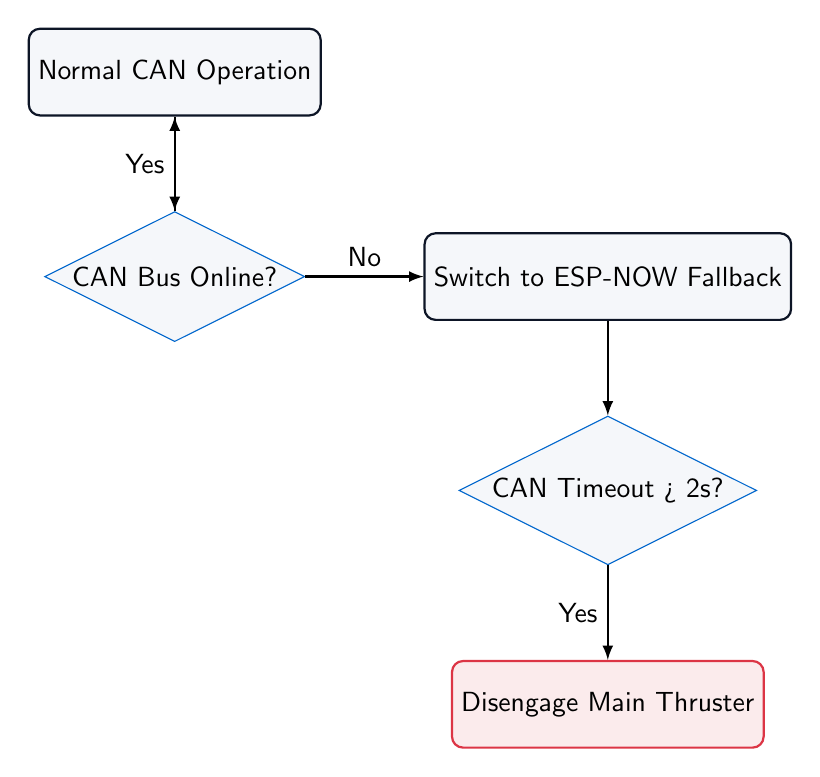
\begin{tikzpicture}[
    node distance=1.2cm and 1.5cm,
    decision/.style={diamond, draw=primaryblue, fill=lightgrey, aspect=2, align=center, inner sep=1pt},
    block/.style={rectangle, draw=darknavy, fill=lightgrey, thick, rounded corners, align=center, minimum width=3.2cm, minimum height=1.1cm},
    alert/.style={rectangle, draw=warnred, fill=warnred!10, thick, rounded corners, align=center, minimum width=3.2cm, minimum height=1.1cm}
]

\node [block] (norm) {Normal CAN Operation};
\node [decision, below=of norm] (can_check) {CAN Bus Online?};
\node [block, right=of can_check] (esp_fb) {Switch to ESP-NOW Fallback};
\node [decision, below=of esp_fb] (wdt_check) {CAN Timeout > 2s?};
\node [alert, below=of wdt_check] (stop) {Disengage Main Thruster};

\path [draw, -latex, thick] (norm) -- (can_check);
\path [draw, -latex, thick] (can_check) -- node[above]{No} (esp_fb);
\path [draw, -latex, thick] (can_check) -- node[left]{Yes} (norm);
\path [draw, -latex, thick] (esp_fb) -- (wdt_check);
\path [draw, -latex, thick] (wdt_check) -- node[left]{Yes} (stop);

\end{tikzpicture}
\caption{System Failsafe Logic Flow for Communication & Motor Safety.}
\label{fig:failsafe_flow_detailed}
\end{figure}

---

% =========================================================
\section{Operational Manual & Maintenance Procedures}
% =========================================================

\subsection{System Startup & Verification Procedure}
\begin{enumerate}
    \item Apply primary power supply (12~V LiPo / 5~V Regulator) to all four ESP32-S3 boards.
    \item Confirm status LEDs transition to steady \textbf{Green}:
    \begin{itemize}
        \item Fast flashing \textbf{Red}: TWAI CAN bus error or wiring open circuit.
        \item Flashing \textbf{White}: MicroSD card initialization failure on Node 3.
        \item Blinking \textbf{Blue}: Active ESP-NOW wireless fallback mode.
    \end{itemize}
    \item Connect PC or mobile browser to Access Point:
    \begin{itemize}
        \item \textbf{SSID:} \texttt{AUV-Control-Station}
        \item \textbf{WPA2 Key:} \texttt{12345678}
    \end{itemize}
    \item Navigate to \url{http://192.168.4.1} to launch the 3D control dashboard.
\end{enumerate}

\end{document}
